\section{Experiments}

\subsection{Experimental Details.}

\noindent
\textbf{Implementation Details.}
%
Our teacher model is initialized with WAN2.2-5B-TI2V~\cite{wan2025wan}.
During streaming distillation, we use an aesthetic scorer as the reward model, with the temperature coefficient $\tau$ set to $0.2$.
% 
During inference, the KV cache size $M=23$. We adopt a chunk-wise generation strategy, where each chunk consists of $3$ latent frames.
% 
All experiments are conducted on NVIDIA A100 GPUs.
% 
Due to space limitations, we provide additional training details in the \textbf{Appendix}.


\noindent
\textbf{Evaluation Settings.}
%
The task most closely related to ours is multi-reference customized video generation. Accordingly, we select several representative baselines: VACE~\cite{vace}, Kaleido~\cite{zhang2025kaleido}, MAGREF~\cite{deng2025magref}, SkyReels-A2~\cite{fei2025skyreels} and Phantom~\cite{liu2025phantom}.
% 
Moreover, we compare with a first-frame editing + Image-to-Video (I2V) pipeline, where Qwen-Image-Edit~\cite{wu2025qwen} performs editing, followed by WAN-5B-TI2V~\cite{wan2025wan} for I2V generation.
Note that all baselines generate videos at their respective native resolutions and durations.
%
To evaluate different methods on the human-garment video customization task, we construct a benchmark termed HGC-Bench.
HGC-Bench contains $240$ samples, each consisting of a reference character image, a garment image, and a corresponding prompt, covering a wide range of characters, scenarios, and garments. We provide additional details in the \textbf{Appendix}.



\begin{table}[!t]
\centering
\caption{
Quantitative comparison of different methods for \textit{short ($81$ frames) video customized generation}. The best results are highlighted in \textbf{bold} and the second best are \uline{underlined}. Note that the frames per second (FPS) of all methods are evaluated on an H200 GPU.
}
\label{tab:main_results}
\small
\setlength{\tabcolsep}{2.5pt}
\begin{tabular}{l c ccccccccc}
\toprule
Methods & Params $\downarrow$ & Cur. $\uparrow$ & GME $\uparrow$ & Amp. $\uparrow$ & Smoo. $\uparrow$ & VQ $\uparrow$ & HGC $\uparrow$ & LGC $\uparrow$ & NTP $\uparrow$ & FPS $\uparrow$ \\
\midrule
Edit~\cite{wu2025qwen}+I2V~\cite{wan2025wan} & 20B+5B & 0.4094 & 0.6741 & \textbf{0.8636} & 0.9898 & \uline{0.7482} & \uline{4.5417} & \uline{3.9167} & 4.4583 & 0.76 \\
VACE~\cite{vace}                             & 14B & 0.2746 & 0.6962 & 0.4054 & 0.9764 & 0.7409 & 4.3708 & 3.5458 & 4.6417 & 0.23 \\
Kaleido~\cite{zhang2025kaleido}              & 14B & 0.3676 & 0.6882 & 0.2675 & \uline{0.9935} & 0.7478 & 4.1708 & 3.5500 & \uline{4.7167} & 0.13 \\
MAGREF~\cite{deng2025magref}                 & 14B & 0.0459 & \textbf{0.7138} & 0.2571 & 0.9436 & 0.7301 & 3.6000 & 2.2000 & 2.6875 & 0.27 \\
SkyReels-A2~\cite{fei2025skyreels}           & 14B & 0.3689 & 0.6550 & 0.5205 & 0.9424 & 0.7241 & 3.3625 &  2.6958 & 4.6458 & 0.54 \\
Phantom~\cite{liu2025phantom}                & 1.3B & \textbf{0.5507} & 0.6855 & 0.1144 & 0.9668 & 0.7338 & 4.3292 & 3.6417 & 4.6875 & \uline{0.77} \\
Phantom ~\cite{liu2025phantom}               & 14B & \uline{0.4911} & \uline{0.6972} & 0.2086 & 0.9932 & 0.7446 & 4.5375 & 3.8333 & 4.6417 & 0.15 \\
\rowcolor{gray!25}
\method     & 5B & \uline{0.4911} & 0.6839 & \uline{0.7771} & \textbf{0.9969} & \textbf{0.7483} & \textbf{4.6833} & \textbf{3.9250} & \textbf{4.7625} & \textbf{23.8} \\
\bottomrule
\end{tabular}
\end{table}



\begin{figure}[t]
    \centering
    
\includegraphics[width=0.98\linewidth]{figures/qualitative.pdf}
    \caption{
    Qualitative comparison of our \method with other baselines.
    % 
    Due to space limitations, we omit the input prompts here; please refer to the Appendix for details.
    }
    \label{fig:qualitative_comparison}
    \vspace{-1.0em}
\end{figure}



\subsection{Main Results}


\noindent
\textbf{Quantitative Comparisons.}
% 
Inspired by prior works~\cite{deng2025magref,liu2025phantom,xue2025stand}, we adopt several evaluation metrics, including ID consistency (Cur Score), text alignment (GME Score), motion magnitude (Amplitude), and temporal smoothness (Smoothness) following OpenS2V-Nexus~\cite{yuan2025opens2v}, as well as overall visual quality (VQ Score) following VBench~\cite{huang2024vbench}.
To assess garment consistency, we use Gemini-3.0 to evaluate the generated results from three aspects: high-level garment consistency (HGC), low-level garment consistency (LGC), and non-target garment preservation (NTP).
In addition, we report the frames per second (FPS) of each method to measure efficiency. See \textbf{Appendix} for details.
% 
In Table~\ref{tab:main_results}, \method outperforms all baselines in temporal consistency, video quality, and three garment consistency metrics.
For ID consistency and motion magnitude, our method ranks second, following the Phantom(1.3B)~\cite{liu2025phantom} and Edit~\cite{wu2025qwen}+I2V~\cite{wan2025wan}, respectively.
\textbf{Notably}, \method significantly outperforms all baselines in efficiency, enabling real-time generation at $23.8$ FPS.



\begin{figure}[t]
    \centering
    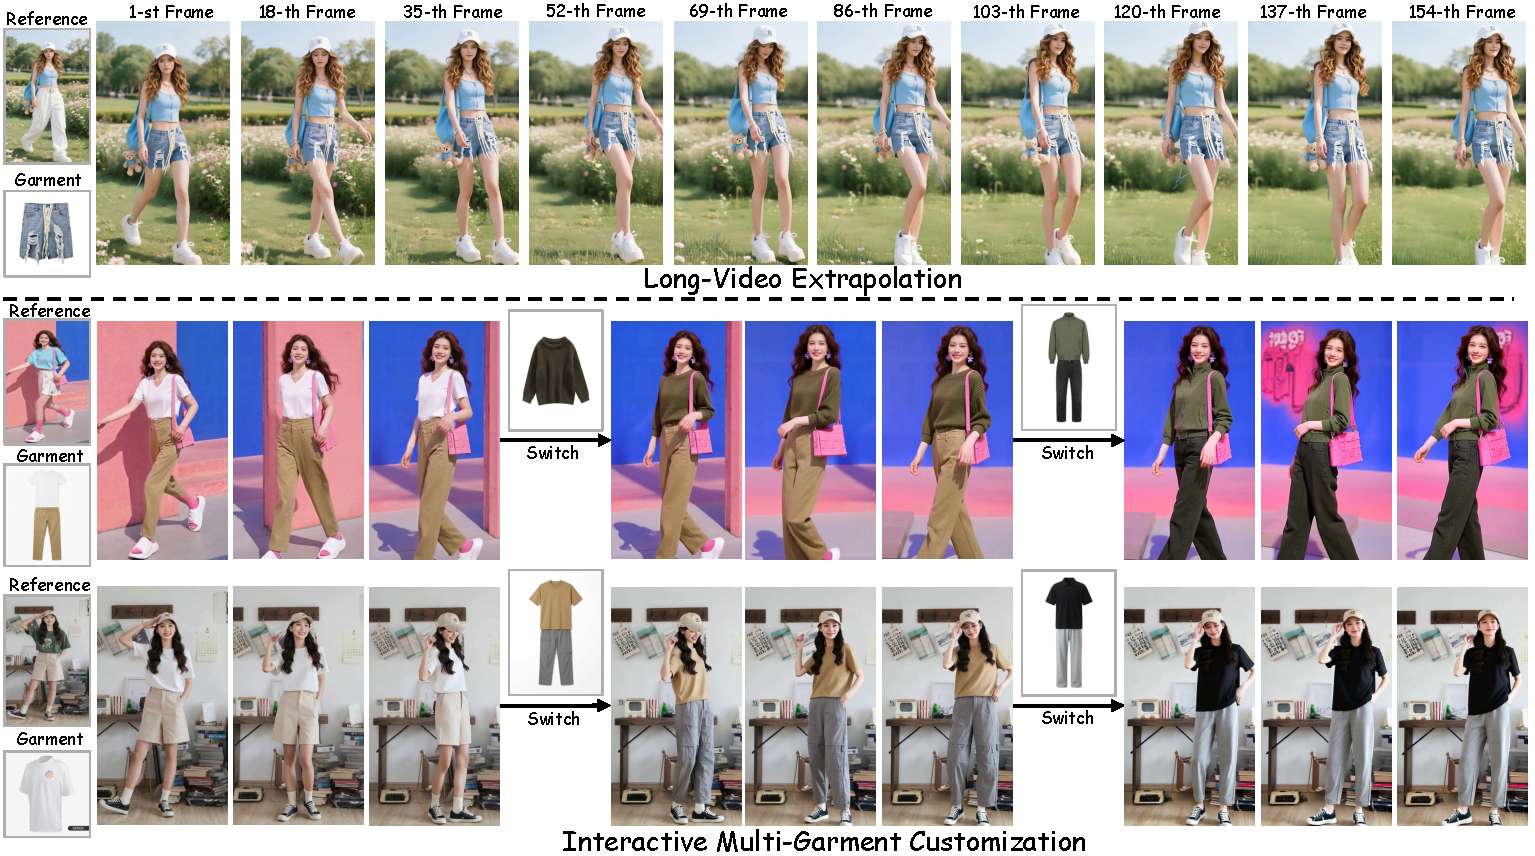
\includegraphics[width=0.98\linewidth]{figures/app.pdf}
    \caption{
    Additional applications of \method. It supports both \textit{long-video extrapolation} and \textit{interactive multi-garment customization}.
    We omit prompts for brevity; see Appendix for details.
    }
    \label{fig:app}
    \vspace{-1.0em}
\end{figure}



\noindent
\textbf{Qualitative Comparisons.}
% 
We further provide qualitative comparisons to assess ID consistency, garment consistency, and overall visual fidelity across different methods. As shown in Figure~\ref{fig:qualitative_comparison}, existing approaches often struggle to simultaneously maintain subject identity, garment details, and natural motions.
% 
In cases involving large pose variations or with complex garments, these methods tend to exhibit noticeable degradation in appearance and garment preservation.
% 
Moreover, several baselines exhibit garment mismatch or unintended modifications to non-target garments, which degrade overall realism and temporal consistency across frames. See \textbf{Appendix} for more results.



\noindent
\textbf{Long-Video Extrapolation.}
% 
Existing multi-reference customization methods rely on bidirectional architectures that synthesize all frames jointly, making them unsuitable for long-video customized generation.
In contrast, the autoregressive generation paradigm of \method naturally supports long-video extrapolation.
% 
As shown in Figure~\ref{fig:app}, \method can maintain character consistency and garment consistency across long temporal ranges. See \textbf{Appendix} for more results.



\noindent
\textbf{Interactive Customization.}
% 
Benefiting from proposed KV Cache Rescheduling, \method further enables interactive multi-garment customized generation, which is beyond the capability of existing methods.
As shown in Figure~\ref{fig:app}, \method supports interactive garment-switching during generation while preserving coherent human motion. See \textbf{Appendix} for more results.



\begin{figure}[t]
    \centering
    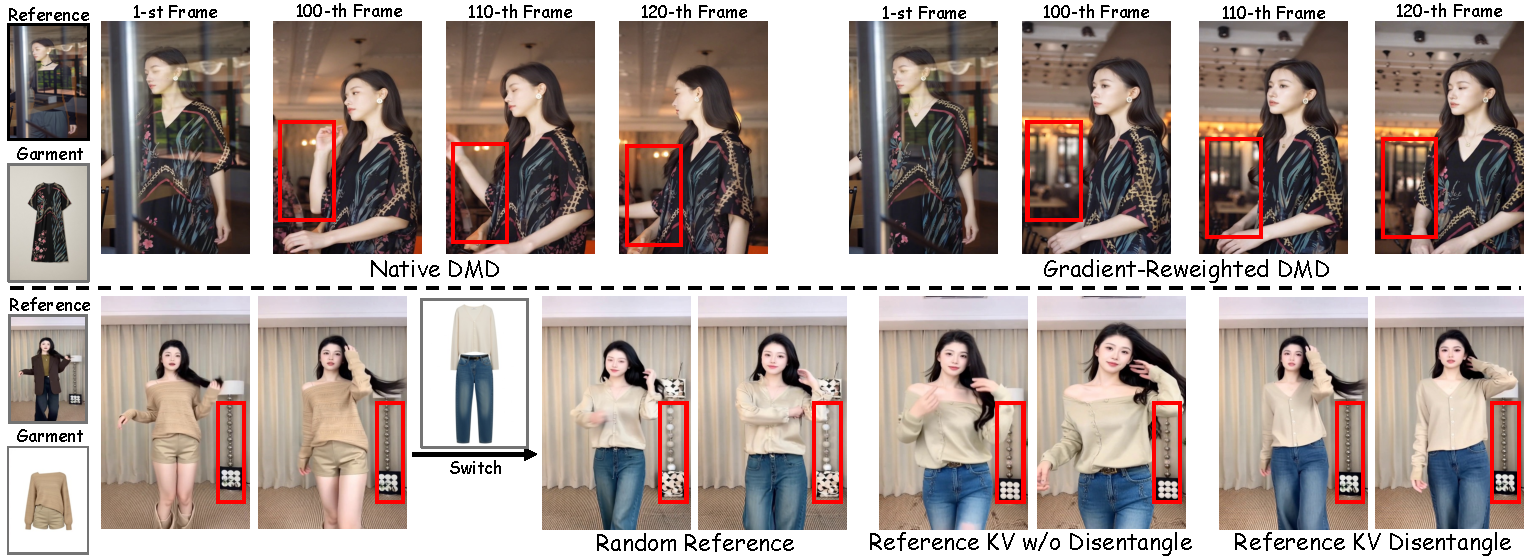
\includegraphics[width=0.98\linewidth]{figures/ablation.pdf}
    \caption{
    Qualitative ablation of \textit{Gradient-Reweighted Distribution Matching Distillation (DMD)} and \textit{Reference KV Disentangle}. 
    % 
    Gradient-Reweighted DMD alleviates motion collapse during extrapolation, while Reference KV Disentangle further enhances consistency during garment switching.
    }
    \label{fig:ablation2}
    \vspace{-1.0em}
\end{figure}



\begin{table}[!t]
\centering
\caption{
Quantitative ablation of teacher training strategies for \textit{short ($81$ frames) video customized generation}. 
% 
The best results are highlighted in \textbf{bold} and the second best are \uline{underlined}.
}
\setlength{\tabcolsep}{3.5pt}
\begin{tabular}{l c ccccccccc}
\toprule
Variants & Cur. $\uparrow$ & GME $\uparrow$ & Amp. $\uparrow$ & Smoo. $\uparrow$ & VQ $\uparrow$ & HGC $\uparrow$ & LGC $\uparrow$ & NTP $\uparrow$ \\
\midrule
Chan.-Concat + Full FT     & 0.1811 & 0.6874 & 0.3748 & 0.9266 & 0.7404 & 4.4917 & 3.1667 & 4.4667 \\
\rowcolor{gray!25}
Ours + Full FT             & \textbf{0.4602} & \textbf{0.6972} & 0.5625 & \textbf{0.9936} & \textbf{0.7473} & \textbf{4.8583} & \textbf{4.1583} & \textbf{4.7792} \\
Ours + Attn FT             & \uline{0.4348} & \uline{0.6900} & \uline{0.6350} & \uline{0.9881} & \uline{0.7471} & \uline{4.8500} & \uline{4.0625} & \uline{4.7750} \\
Ours + LoRA~\cite{hu2022lora} FT               & 0.4046 & 0.6928 & \textbf{0.6448} & 0.9777 & 0.7437 & 4.7292 & 3.9458 & 4.7042 \\
\bottomrule
\label{tab:ablation1}
\vspace{-1.0em}
\end{tabular}
\end{table}



\begin{table}[!t]
\centering
\caption{
Quantitative ablation of Gradient-Reweighted Distribution Matching Distillation (GR-DMD) for \textit{long ($165$ frames) video customized generation}. The best results are highlighted in \textbf{bold}.
}
% \small
\setlength{\tabcolsep}{2.5pt}
\begin{tabular}{l c ccccccccc}
\toprule
Variants & Cur. $\uparrow$ & GME $\uparrow$ & Amp. $\uparrow$ & Smoo. $\uparrow$ & VQ $\uparrow$ & HGC $\uparrow$ & LGC $\uparrow$ & NTP $\uparrow$ \\
\midrule
Naive DMD           & 0.4232 & 0.6700 & 0.8026 & 0.9932 & 0.7419 & 4.6958 & 3.8958 & 4.7125  \\
\rowcolor{gray!25}
GR-DMD ($\tau=0.2$) & \textbf{0.4265} & 0.6732 & \textbf{0.8395} & \textbf{0.9975} & \textbf{0.7480} & 4.7000 & 3.9042 & \textbf{4.7333}  \\
GR-DMD ($\tau=0.3$) & 0.4111 & \textbf{0.6786} & 0.5106 & 0.9933 & 0.7465 & \textbf{4.7583} & \textbf{3.9375} & 4.6958  \\
GR-DMD ($\tau=0.4$) & 0.4047 & 0.6696 & 0.7869 & 0.9872 & 0.7424 & 4.7125 & 3.9022 & 4.7208  \\
GR-DMD ($\tau=0.5$) & 0.4252 & 0.6774 & 0.7907 & 0.9953 & 0.7421 & 4.7083 & 3.8833 & 4.7058  \\
\bottomrule
\label{tab:ablation2}
\vspace{-1.0em}
\end{tabular}
\end{table}



\subsection{Ablation Studies}
%
In this section, we conduct three groups of ablation studies: \textit{Teacher Model}, \textit{Streaming Distillation}, and \textit{KV Cache Rescheduling}.
% 
Additional ablation results are provided in the \textbf{Appendix}.



\noindent
\textbf{Ablation with Teacher Model.}
% 
To validate the effectiveness of \textit{In-Context Learning}, we compare it with channel-wise concatenation.
In Table~\ref{tab:ablation1}, our designed in-context learning outperforms simple channel-wise concatenation across several metrics.
% 
Moreover, we compare different fine-tuning (FT) strategies, including Full FT, Attn FT, and LoRA~\cite{hu2022lora} FT, with the results shown in Table~\ref{tab:ablation1}.
% 
Full FT performs best overall, so we adopt this version of the teacher model for streaming distillation.



\noindent
\textbf{Ablation with Streaming Distillation.}
% 
We first analyze the effectiveness of \textit{Gradient-Reweighted Distribution Matching Distillation (GR-DMD)} in long-video (165 frames) extrapolation through qualitative and quantitative evaluations, as shown in Table~\ref{tab:ablation2} and Figure~\ref{fig:ablation2}.
% 
Intuitively, naive DMD tends to produce distorted or duplicated human limbs during extrapolation.
% 
In contrast, our Gradient-Reweighted DMD generates coherent and anatomically consistent human structures during extrapolation.
% 
Moreover, we further investigate the effect of the temperature coefficient $\tau$ on long-video extrapolation.
% 
In Table~\ref{tab:ablation2}, the hyper-parameter $\tau=0.2$ yields the best overall performance.



\noindent
\textbf{Ablation with KV Cache Rescheduling.}
% 
We now analyze the choice of reference KV and the effectiveness of disentanglement, as visualized in Figure~\ref{fig:ablation2}.
% 
Clearly, randomly selecting reference KV leads to inconsistencies with previous frames.
This phenomenon stems from the image-to-video prior, where the generated initial frame aligns with the reference image; thus, mismatched reference KV breaks temporal coherence.
% 
Moreover, without disentangling the last historical KV, distribution mismatch arises: the reference frame is independently VAE-encoded during training, while the non-disentangled historical KV corresponds to multiple decoded frames (\emph{e.g.}, four).
